%-----------------------------------------------------------------------------%
\chapter{\topikTiga}
%-----------------------------------------------------------------------------%

%-----------------------------------------------------------------------------%
\section{Pendahuluan}
%-----------------------------------------------------------------------------%
	Conjugate gradient method digunakan untuk menyelesaikan persamaan linear $Ax = b$ di mana matriks koefisiennya bersifat simetris dan definit positif.  Matriks $A$ $n$ x $n$ dikatakan simetris jika $a_{ij}$ = $a_{ji}$ untuk $i,j = 1,...,n$.  Matriks $A$ dikatakan definit positif jika untuk setiap vektor $x$ bukan nol, perkalian skalar $x \cdot Ax$ menghasilkan nilai lebih besar dari nol.
	Algoritma conjugate gradient method ditunjukkan pada \pic~\ref{fig:cg}.  $r_{k}$ merupakan sisa atau selisih antara $b$ 
	dengan $Ax_{k}$, sedangkan $p_{k}$ merupakan \f{search direction}.
	
	\begin{figure}
		\centering
		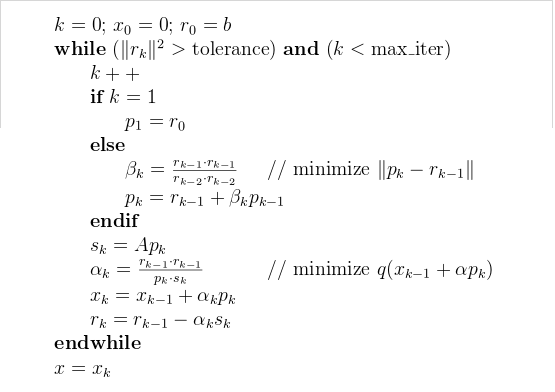
\includegraphics[width=0.75\textwidth]
			{pics/cg_par.png}
		\caption{Algoritma Conjugate Gradient Method.}
		\label{fig:cg}
	\end{figure}  
	
	Pada implementasi paralel CGM, matriks $A$ akan didistribusikan menggunakan fungsi \texttt{MPI\_scatter} kepada setiap proses dan masing-masing proses mendapat sebanyak $n$ x $n$ / $p$ data.  Algoritma tersebut dijalankan di setiap proses untuk setiap bagian distribusi matriks $A$.
%-----------------------------------------------------------------------------%
\section{Eksperimen}
%-----------------------------------------------------------------------------%

\todo{}

%-----------------------------------------------------------------------------%
\section{Kesimpulan}
%-----------------------------------------------------------------------------%

\todo{}
